% 
%   How I want to get to the Solution and why I choosed it also how it works.
%   Also there should be some theory about state estimation and the kalmanfilter used
%   in this
%   
%   \section{Tipps/Notes}
%   - Don't forget point of origin / reference system
%   - Don't forget the pitch angle
%   Maybe do rocket model here
 
  
  \section{Verification}
  First of all the test concept has to be defined on which the developed algorithms will be tested.
  For this the following concept figure \ref{fig:Verification} was developed.
  
  \begin{figure}[h!]
   \centering
   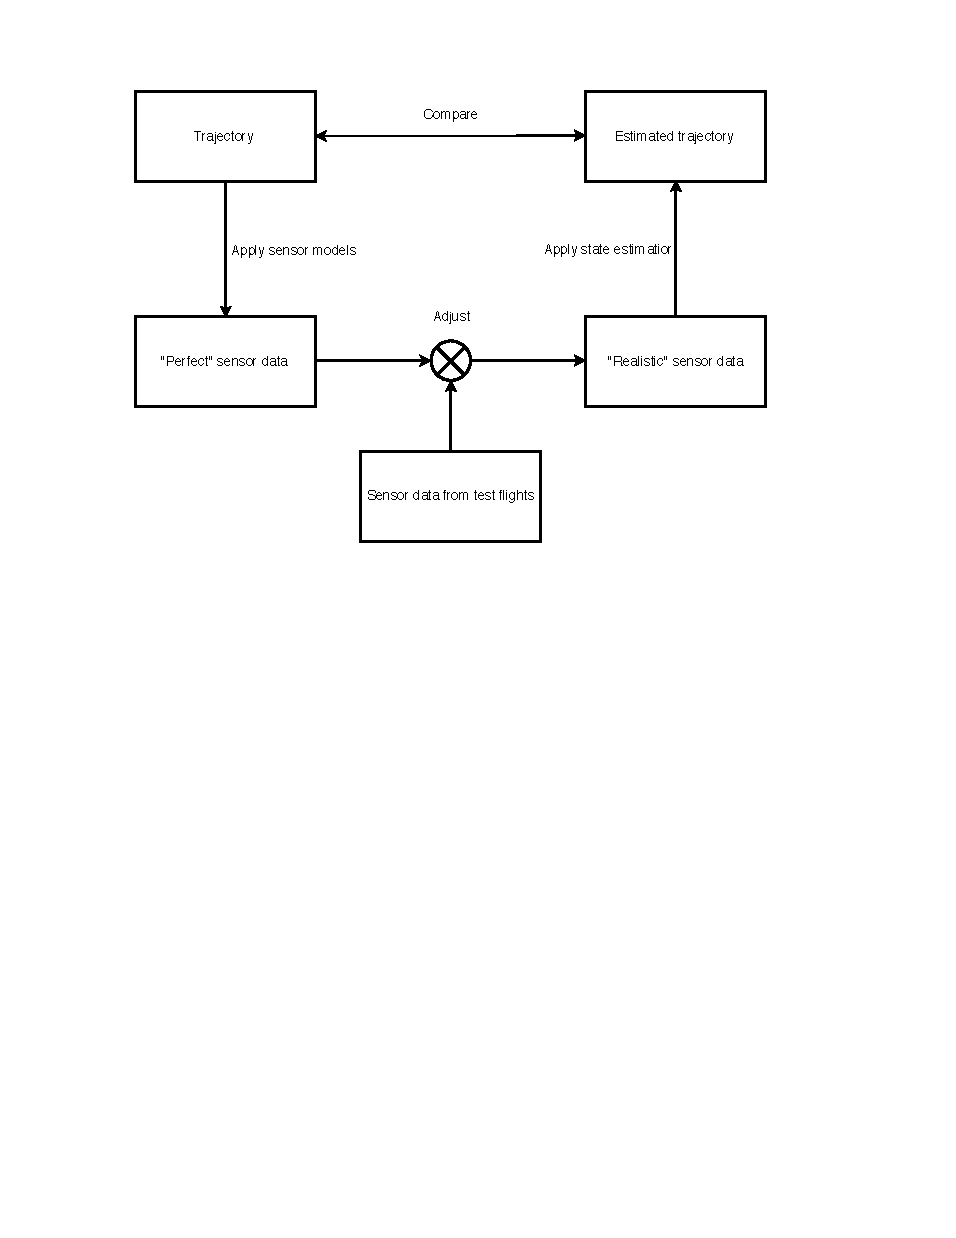
\includegraphics[width = \textwidth]{../BDADoku/Pictures/Verification.pdf}
   \caption{Verification Concept}
   \label{fig:Verification}
  \end{figure}

  The theory behind this is that a trajectory is generated by the simulation, which should resemble a real trajectory as good as possible.
  This function was provided by the simulation team of ARIS from the last years competition.
  Then this trajectory is applied on the sensor models which are developed in chapter \ref{ch:Implementation}.
  This generates so called perfect sensor data. 
  After this the noise is applied which will also be developed later in this chapter, which will result in real sensor data. 
  This noise is drawn out of the sensor log data from the previous test flights.
  After the realistic sensor data is generated, it serves as the input to the different estimation algorithms.
  
  Then to verify the functionality of those algorithms, the estimated trajectory is then compared against the generated trajectory.
  
  
  \section{Sensor models}
  As stated above the trajectory will be generated by the simulation. 
  This are just the information of the height, so the different sensor models have to be adjusted to get to the different needed data.
  The models are defined as follow.
  
  \subsection{Accelerometer}
  Perfect measuring from the accelerometer is in simple terms the two times deviation of the height.
  $$a = \frac{d^2h}{dt^2}$$
  This equals in the straight up acceleration. To get the acceleration which would be provided by an accelerometer,
  the pitch angle has to be calculated into this generated data.
  
  \subsection{Gyrometer}
  The gyrometer data can not be directly calculated out of the simulated height.
  Therefore it has to be generated separately.
  For this the gyrometer data from the test flights will be taken into account.
  
  \subsection{Barometer}
  The barometer which are used in the aerospace usually provide the pressure in hecto Pascal as well as the temperature in degree Celsius.
%   -Use density as a statevector \\
%   -Use exponential atmosphere method. \\
%   -Increasing the R measurement noise matrix when rocket is ascending access the rising uncertainties
  \subsubsection{Pressure}
  To generated the pressure data, the international atmospheric model is used %Hier Internet Referenz einfügen
  $$P = P0 * (1- \frac{TCoeff*h}{T0})^{5.255}$$
  with: PO = Pressure at sea level \\
	TO = Temperature at sea level
  This is more or less accurate till 30 000 meter under the condition that the Temperature coefficient is determined correct. 

  \subsubsection{Temperature}
  The temperature depending on the height is difficult to calculate.
  This due to a lot of uncertainties on which the temperature is depending.
  For example different air currents and air holes...
  The mean TCoeff is stated as -0.0065 degree Celsius per meter.
  $$T = T0 - TCoeff*h$$
  
  \subsection{GPS}
  The perfect GPS data is seen as the accurate height but with a slow sample rate around 0.5 to 2 Hz.
  This can simply be achieved by downsampling the height vector with the right factor.
  
  
  \section{Noise generation}
  To generate the different noises, first the noise from the test flight has to be extracted.
  If done so, a system can be calculated which represents a white noise filter that generates noises
  that has the same spectral power density as original noise. This process is visualised in figure.
  
  %% Bild vom white noise filter conzept einfügen
  
  
  For this the yule walker equation should come in handy to generate a so called AR (auto regressive) model of the noise system.
  But to get the correct coefficients, the noise has to have a steady mean value preferably it should be zero mean.  
  
  \section{State estimator}
  Which ones are there and what are their positives and negatives, in short how do they work
  I will use kalman filter with time depending system and sensor noise, but i have yet to define how i do this in peticullar.
  I should also make some pictures and such things.
  
  There are many possibilities to do sensor fusion. first of all an all new algorithm could be developed which accesses the 
  stated problems directly. While this solution would be preferable regarding the efficency, the 
  time ad knowledge needed for this task would exceed the resoursces given in this thesis by far.
  Also as stated in chapter \ref{ch:Introduction} a lot of theoretical as well as practical pre work is
  already done and therefore should be used. 
  
  \subsection{Kalmanfilter}
  
  \begin{figure}[h!]
  \centering
  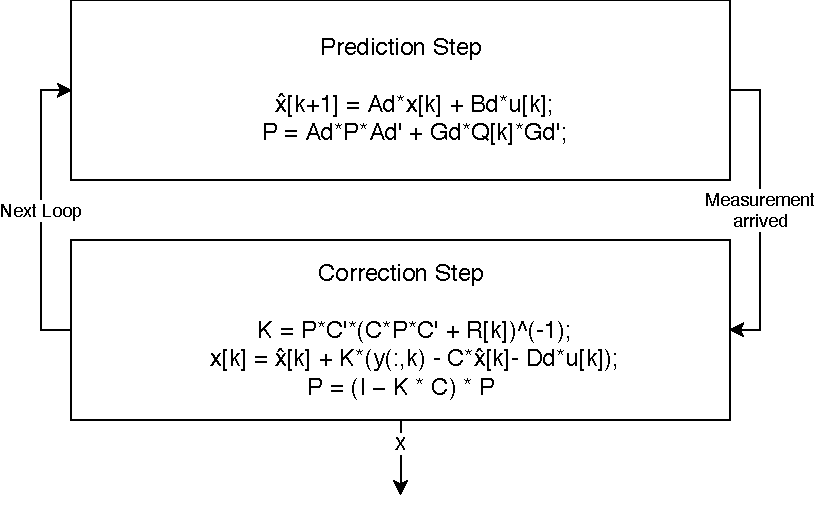
\includegraphics[width = \textwidth]{../BDADoku/Pictures/KalFIlFunc.pdf}
  \caption{Kalmanfilter}
  \label{fig:Kalmanfilter}
  \end{figure}
 
  The discrete Kalmanfilter figure \ref{fig:Kalmanfilter} was first introduced by Kalman in the year 1960.
  Its structure provides the optimal estimation of the standard deviation estimation error as long as the noise is Gaussian.
  But there lies the problem, a physical system is most often not linear.
  Also the estimated system as well as its variances over the time have to be known to provide this optimal estimation.
  If the noise matrices of the system are static, the filters gain matrices aim for a fix value and can therefore be calculated in beforehand.
  This reduces the computational effort by a significant amount. \cite{DavidWSchultz2004}.
  It should be mentioned that even if the noise is not Gaussian, the kalmanfilter is still the best
  linear estimator as long as the system and its properties are well known \cite{SimonDan2006Ose:}.
  
  \subsection{ROSE}
  The ROSE(rapid ongoing stochastic estimator) is in simple terms three kalman filters in one.
  Where the main filter is used as stated above, the additional two are used to estimated the 
  the system noise as well as the measuring noise. Therefore this sensor preforms better than the traditional kalman filter
  if those noises change over time in a not known fashion and has therefore be estimated.
  Due to this, this sensor needs more computational effort \cite{DavidWSchultz2004}. 
  
  \subsection{Extended Kalmanfilter}
  The extended kalmanfilter provides additional parts to better access nonlinearity in the observed system.
  This by not estimating the state of the system but by estimating the linearized change of the state 
  to the past sate. For this the systems equations have to be derived around the current working point in every estimation state.
  This is some sort of Bootstrap solution because the nominal point on which the derivation happens are estimated in the process and
  this estimates are then used to estimate the change between this estimation and the next.
  Therefore the computational effort exceeds even further \cite{SimonDan2006Ose:}.
  
  \subsection{Unscented Kalmanfilter}
  The unscented kalmanfilter takes the unscented transformation in use to calculate the different interpolating steps.
  The unscented transformation uses different points on which the mean and the covariance of a state is known to estimate the 
  change in the next iteration much better than the normal linearized approach.
  But for this the unscented Kalmanfilter needs also to apply the unscented transformation onto the state vectors in each iteration
  and does therefore need even more computational effort.
  
  \subsection{H$\infty$ filter}
  The H$\infty$ filter is a more diverse approach then the ones described above.
  It was developed to access the problem when the to be observed system espacially its noise is not well known.
  Also in contrast to the kalman filters the H$\infty$ filter minimizes the worst-case estimation error 
  in stand of the standard deviation of the estimation error.
  
  \section{Choosing}
  If the requirements table \ref{tab:Requirements} is taken into the consideration of finding
  the optimal solution, two main requirements occur that define this decision.
  First the system load is a critical requirements and has therefore to be addressed in this process.
  Also for the requirement of modularity the algorithm should be as simple as possible.
  If taken in regard that the system is more or less well known and that the noise can be
  determened with the simulation and the log data from previous test flights,
  a normal kalmanfilter seems to be the most fitting solution.
  This because the performance of the rocket and the sensor should stay the same during
  each flight. 
  
  \section{System Model}
  The system model to represent the rocket
  will be hold simple to reduce the system load as well as prevent nonlinearities.
  Also the important values to estimate are at first hand the vertical height and speed, so
  for a first implementation just variables that can bed used do determine those both will be used.
  This are mainly the height and speed from the GPS, the vertical acceleration from the accelerometer
  as well as the pressure and temperature from the pressure sensors.
  But even with such simplification there are different possible system description which have to be taken into account 
  to find the best suitable.
  
  \subsection{Point Mass}
  The most simple possible model would be, that the rocket would be resembled as a simple point mass which flies perfectly vertical upwards.
  For this only three state variables would be necessary, the vertical acceleration, the vertical speed and the height.
  $$x = \begin{bmatrix}
  h_z\\
  v_z\\
  a_z
  \end{bmatrix} $$ 
  This would reduce the dynamics matrix of the system to a 3x3 matrix with with only two 1 in it:
  $$ A = \begin{bmatrix}
  1 & 0 & 0\\
  0 & 1 & 0\\
  0 & 0 & 0
  \end{bmatrix} $$ 
  As normal in engineering such a simplification comes with a cost. With this system description the output from the barometer would have
  to be transformed into the height before they could be taken into the system. 
  Due to this the properties of these sensor could not be estimated correct because the value was transformed in a non linear way before it entered the system.
  In addition the same problem occurs with the accelerometer. If the rocket develops a pitch angle not equal to 0 during the asccending, it would be measured wrong.
  To counter this error, the measurements of the accelerometer would have to be weighted with the angle of the gyrometer before entering the system.
  This weighting is also non linear and the values of the gyrometer are not filtered, which would make the estimation even more uncertain.
  
  \subsection{Point Mass with Pressure and Temperature}
  To taken into account to problem stated above, pressure and temperature can be taken into the state vector and therefore be estimated.
    $$ x = \begin{bmatrix}
  h_z\\
  v_z\\
  a_z\\
  p\\
  T
  \end{bmatrix} $$ 
  While this solves the problem stated above, it also produces a new. The system model can only describe linear dependencies between the state variables,
  but the relation between the pressure and the height is clearly non linear in each atmospheric model.
  This dependency can be linearized, but if done so, it does resemble the athmosperic model with less accuracy.
  This as to be taken into account an has to be 'told' to the state estimator.
  The change of the temperature depending on the height is a difficult manor.
  But to make it simple I use $KT_h$ =  -0.0065 °/m in this.
  
  This results in a 5x5 dynamic system matrix which looks like this:
  $$ A = \begin{bmatrix}
         1    & 0 & 0 & 0    & 0 \\
         0    & 1 & 0 & 0    & 0 \\
         0    & 0 & 0 & 0    & 0 \\
         KP_h & 0 & 0 & KP_T & 0 \\
         KT_h & 0 & 0 & 0    & 0 
        \end{bmatrix} $$
  
  \subsection{Point Mass with Angle, Pressure and Temperature}
  The same solution as above can also be applied for the pitch angle. The linearization of small angle changes in the sinus is the angle itself.
  The assumption that the pitch angle of the rocket wont be to great during the ascention is suitable due to its flight caracterices.
  This would change the state vector from above into the following.
      $$ x = \begin{bmatrix}
  h_z\\
  v_z\\
  a_z\\
  \varphi_{pitch}\\
  p\\
  T
  \end{bmatrix} $$
  
  But now how to do this ?
  describe here how the system description looks in particular 
  
  
  Those described different system will no be implemented in matlab to find the best possible.

